\documentclass[aspectratio=1610]{beamer}
\hypersetup{
        unicode=true,
        linkcolor=blue,
        anchorcolor=blue,
        citecolor=green,
        filecolor=black,
        urlcolor=blue
    }

%%%%% PACKAGES HERE
%% \usepackage{}
\usepackage{amsmath}
\usepackage{amssymb}
\usepackage{listings}
\usepackage[cache=false]{minted}
\usepackage{textcomp}
\usepackage{tabularx}
\usepackage{algpseudocode}

\usepackage[style=authortitle,backend=biber]{biblatex}
\addbibresource{references.bib}

%%%%%%%%%%%%%%%%%%%%%%%%%%%%%%%%%%%
%% DO NOT CHANGE

\usetheme{default}
\useinnertheme{circles}
\useoutertheme{infolines}
\usefonttheme{serif}

\usepackage{etoolbox}

%% T for navigation symbols
%%\setbeamertemplate{navigation symbols}{}

%% T for header
%% \setbeamertemplate{headline}{%
%%   \leavevmode%
%%   \ifdefempty{\insertsubsectionhead}{
%%     \begin{beamercolorbox}[wd=0.99\paperwidth,ht=2.25ex,dp=1ex,center]{section in head/foot}%
%%       % \hbox to .5\paperwidth{\hfil\insertsectionhead\hfil}
%%       \insertsectionhead
%%     \end{beamercolorbox}%
%%   }{
%%     \begin{beamercolorbox}[wd=.44\paperwidth,ht=2.25ex,dp=1ex,right]{section in head/foot}%
%%       % \hbox to .5\paperwidth{\hfil\insertsectionhead\hfil}
%%       \insertsectionhead
%%     \end{beamercolorbox}%
%%     \begin{beamercolorbox}[wd=.1\paperwidth,ht=2.25ex,dp=1ex,center]{section in head/foot}%
%%       % \hbox to .5\paperwidth{\hfil\insertsectionhead\hfil}
%%       -
%%     \end{beamercolorbox}%
%%     \begin{beamercolorbox}[wd=.44\paperwidth,ht=2.25ex,dp=1ex,left]{subsection in head/foot}%
%%       % \hbox to .5\paperwidth{\hfil\insertsubsectionhead\hfil}
%%       \insertsubsectionhead
%%     \end{beamercolorbox}
%%   }%
%% }

%% T for frame title
\setbeamertemplate{frametitle}{%
  \usebeamerfont{frametitle}\insertframetitle\strut%
  \vskip-0\baselineskip%
  \leaders\vrule width .95\paperwidth\vskip1pt%
  \vskip0pt%
  \nointerlineskip
}

%% T for footer
\setbeamercolor{footlinecolor}{fg=cyan,bg=green}
\setbeamercolor{author in head/foot}{fg=blue}

\setbeamertemplate{footline}{%
  \leavevmode%
  \hbox{%
  \begin{beamercolorbox}[wd=.26\paperwidth,ht=2.25ex,dp=1ex,left]{author in head/foot}%
    \hspace*{2ex}\usebeamerfont{author in head/foot} DS-MSSP22
  \end{beamercolorbox}%
  \begin{beamercolorbox}[wd=.50\paperwidth,ht=2.25ex,dp=1ex,center]{author in head/foot}%
    \usebeamerfont{title in head/foot}Supervised Learning
  \end{beamercolorbox}%
  \begin{beamercolorbox}[wd=.24\paperwidth,ht=2.25ex,dp=1ex,right]{date in head/foot}%
    \usebeamerfont{date in head/foot}
    \insertshortdate{}\hspace*{1em}  % date
    \insertframenumber/\inserttotalframenumber\hspace*{2ex}
  \end{beamercolorbox}}%
  \vskip0pt%
}
%%%%%%%%%%%%%%%%%%%%%%%%%%%%%%%%%%%%%%%%%%%%%%%%

%% Start from here.
\title{Supervised Learning}
\author{Data Science - MASSP 2022}
\date{}

\begin{document}

\begin{frame}[plain]
  \titlepage
\end{frame}


\begin{frame}{Outline}
  \tableofcontents
  \end{frame}

\section{Supervised Learning setup}

\begin{frame}{Supervised learning setup}

\begin{minipage}{0.6\textwidth}
Training data comes in pairs of inputs ($x$,$y$), $x$ $\in$ $\mathbf{R}^d$ is the input, and $y$ its label.\\
$D = \{(x_1,y_1), ..., (x_n,y_n))\} \subseteq \mathbf{R}^d \times C$
  \begin{itemize}
      \item $\mathbf{R}^d$ is the d-dimensional feature space.
      \item $x_i$ is the input vector of the $i^{th}$ sample.
      \item $y_i$ is the label of the $i^{th}$ sample.
      \item $C$ is label space.
  \end{itemize}
  The data points $(x_i,y_i)$ drawn from some (unknown) distribution $P$.\\ We would like learn a function $f$ such that for new pair $(x,y) \sim P$, we have $f(x) = y$ with high probability.
  
\end{minipage}
\begin{minipage}{0.35\textwidth}
    \begin{figure}[h!]
  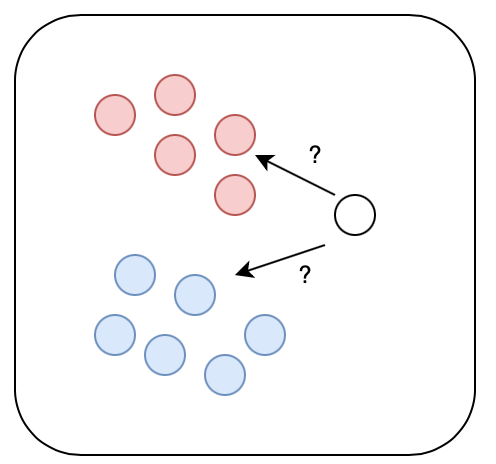
\includegraphics[width=0.6\textwidth]{supervised_learning_setup.png}
  \caption{Supervised Learning}
  \label{fig2}
\end{figure}
\end{minipage}


\end{frame}


\begin{frame}{Feature vectors and label spaces}
1. Label spaces\\
\begin{center}
\begin{tabular}{|c|c|c|} 

 \hline
 Binary classification & $C$ = \{-1,+1\} & e.g. spam filtering\\ 
 \hline
 Multi-class classification & $C$ = \{1,2,...K\}, K $>$ 2 & e.g. face classification\\
 \hline
 Regression & $C = \textbf{R}$ &  e.g. house price prediction \\
 \hline
\end{tabular}
\end{center}
    
2. Feature vectors
\begin{itemize}
    \item Patient data in hospital: $x_i = (x_i^1, x_i^2,...,x_i^d)$, $x_i^1$ refer to the patient's gender, $x_i^2$ could be height of patient in cm, ...
    \item House price data: $x_i = (x_i^1, x_i^2,...,x_i^d)$, $x_i^1$ refer to the area of the house, $x_i^2$ could be the number of bedrooms, ...
\end{itemize}
    
\end{frame}

\section{k-NN algorithm}

\begin{frame}{K-NN algorithm}
\begin{minipage}{0.6\textwidth}
\underline{Assumption}: Similar inputs have similar outputs.\\
\underline{Classification rule}: for a test $x$, assign the most common label amongst its k most similar training inputs.\\
\underline{More formulate}:
\begin{itemize}
    \item Test point $x$
    \item The set of k nearest neighbors of $x$ is $S_x$, \\$S_x\subseteq D$ s.t. $|S_x| = k$ and $\forall (x',y') \in D\setminus S_x$
    
\end{itemize}
 $$\textbf{dist}(x,x') \geq \mathbf{max}_{(x'',y'')\in S_x} \textbf{dist}(x,x'')$$
Define a function $f$ returning the most common label in $S_x$
$$f(x) = \textbf{mode}({y'':(x'',y'') \in S_x})$$
\textbf{mode(.)} means to select the label of highest occurrence.
  
\end{minipage}
\begin{minipage}{0.3\textwidth}

    \begin{figure}[h!]
  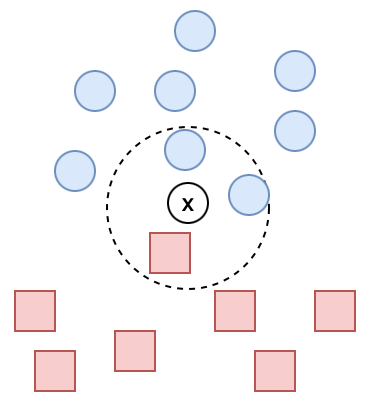
\includegraphics[width=0.6\textwidth]{Screen Shot 2022-05-21 at 14.44.10.png}
  \caption{A binary classification with k = 3. #QUIZ: k = n? k = 1?}
\end{figure}
\end{minipage}
\end{frame}

\begin{frame}{Distance functions}
    The Minkowski distace
    $$\textbf{dist}(x,x') = \Bigg(\sum_{r=1}^{d}|x_r - x'_r|^p\Bigg)^{1/p}$$
  \begin{itemize}
      \item $p = 1$ (norm 1): $\textbf{dist}(x,x') = |x_1 - x'_1| + |x_2 - x'_2| + ... + |x_d - x'_d|$
      
      \item $p = 2$ (norm 2): $\textbf{dist}(x,x') = \sqrt{|x_1 - x'_1|^2 + |x_2 - x'_2|^2 + ... + |x_d - x'_d|^2}$
      \item $p\to 0, p\to\infty$
  \end{itemize}  
  \begin{figure}[h!]
  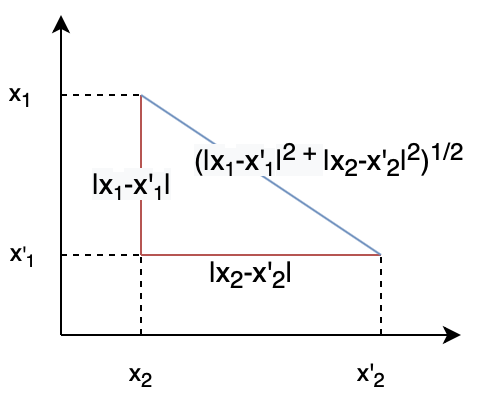
\includegraphics[width=0.36\textwidth]{Screen Shot 2022-05-21 at 16.33.12.png}
\end{figure}
  
  
\end{frame}

\section{The Perceptron}

\begin{frame}{The Perceptron}

 \underline{Assumptions}
 \begin{itemize}
     \item Binary classification (i.e. $y_i \in \{-1,+1\}$)
     \item Data is linearly separable
 \end{itemize}
 
\underline{Classifier}: h(x_i) = sign(W^Tx_i + b)

\begin{figure}[h!]
  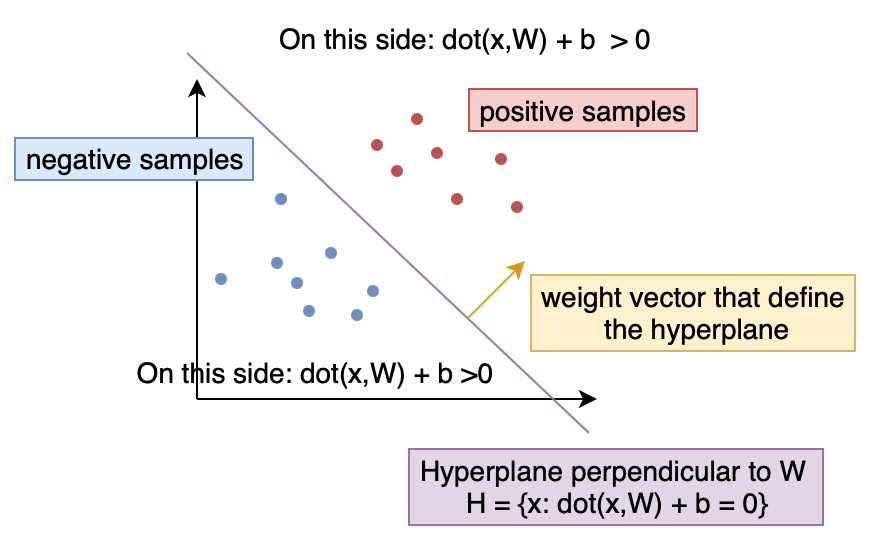
\includegraphics[width=0.45\textwidth]{Screen Shot 2022-05-21 at 19.16.23.png}
\end{figure}
 
\end{frame}
\begin{frame}{The perceptron (cont.)}
\begin{itemize}
    \item $b$ is the bias term, without bias term, the hyperplane always have to go through the origin.
    \item $x_i \gets$  \begin{bmatrix}
       x_i\\
       1
     \end{bmatrix}, $W \gets$  \begin{bmatrix}
       W\\
       b
     \end{bmatrix}
     \item 
      $\begin{bmatrix}
       x_i\\
       1
     \end{bmatrix}^T$\begin{bmatrix}
       W\\
       b
     \end{bmatrix} = $W^Tx_i + b$
     
     \item $h(x_i) = sign(W^Tx_i)$
\end{itemize}



\end{frame}
\begin{frame}{The Perceptron (cont.)}
    \begin{figure}[h!]
  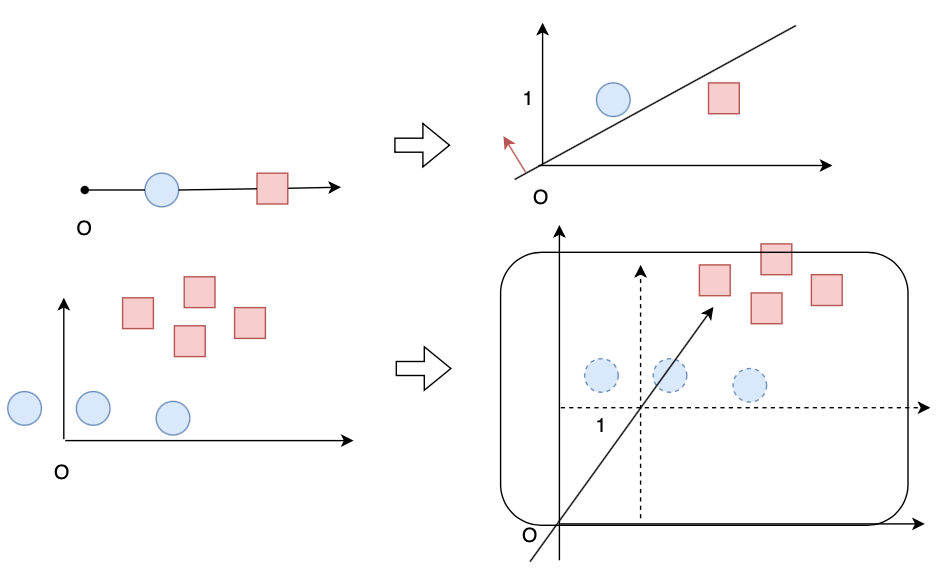
\includegraphics[width=0.6\textwidth]{Screen Shot 2022-05-21 at 20.31.58.png}
  
\end{figure}
\begin{itemize}
    \item Left figure: There is no hyperplane that through the origin and separates data points.
    \item Right figure: After adding constant dimension, the hyperplane exists.
    \item Note that: $y_i(W^Tx_i) > 0 \iff x_i$ is classified correctly. 
\end{itemize}
\end{frame}

\begin{frame}{The Perceptron (cont.)}
    The Perceptron Algorithm
    \begin{algorithmic}
\State Initialize $\Vec{w} = \Vec{0}$ \Comment{Misclassifies everything}
\While{true}
    \State $m \gets 0$ \Comment{count the number of miss classifications}
    \For{$(x_i,y_i) \in D$}
        \If{$y_i(\Vec{w^T}.\Vec{x_i}) \leq 0$} \Comment{If mis classification}
            \State $\Vec{w} \gets \Vec{w} + y\Vec{x}$ \Comment{update the weight vector}
            \State $m \gets m + 1$ \Comment{count the number of misclassifications}
        \EndIf
    \EndFor
    \If{$m = 0$}
        \State break
    \EndIf
\EndWhile

\end{algorithmic}
    
\end{frame}

\begin{frame}{The Perceptron (cont.)}

Geometric Intuition
     \begin{figure}[h!]
  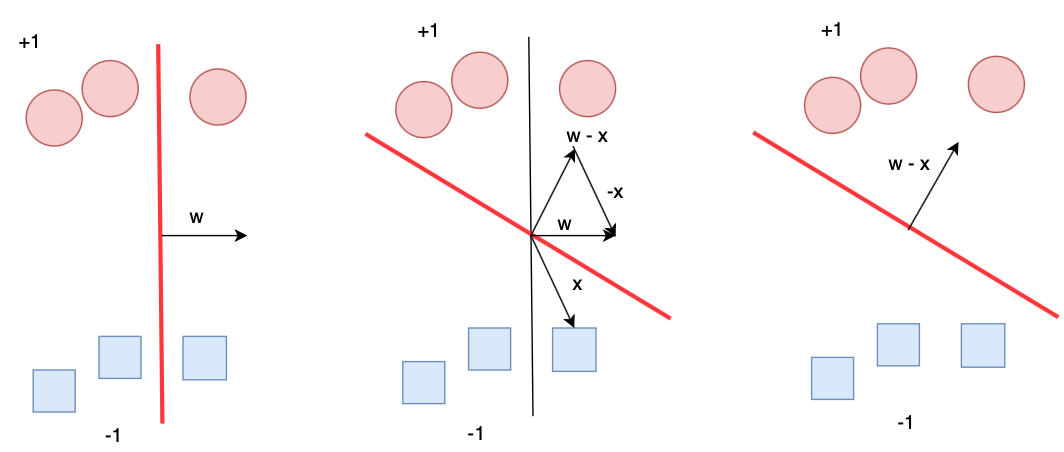
\includegraphics[width=0.75\textwidth]{Screen Shot 2022-05-21 at 21.20.43.png}
  \caption{Illustration of a perceptron update}
  
\end{figure}
\end{frame}

\begin{frame}{Perceptron Convergence}
    If the data is linearly separable, the Perceptron will find a separating hyperplane in a finite number of updates.
    \begin{itemize}
        \item The argument: Suppose $\exists w^*$ such that $y_i(x^Tw^*) > 0$ $\forall (x_i,y_i) \in D$
        \item Suppose: rescale each data point and the $w^*$ such that: $||w^*|| = 1$ and $||x_i|| < 1$ $\forall x_i \in D$
        \item Margin $\gamma$ of the hyperplane $w^*$ as $\gamma = min_{(x_i,y_i)\in D}|x_i^Tw^*|$
    \end{itemize}
    
    \begin{figure}[h!]
  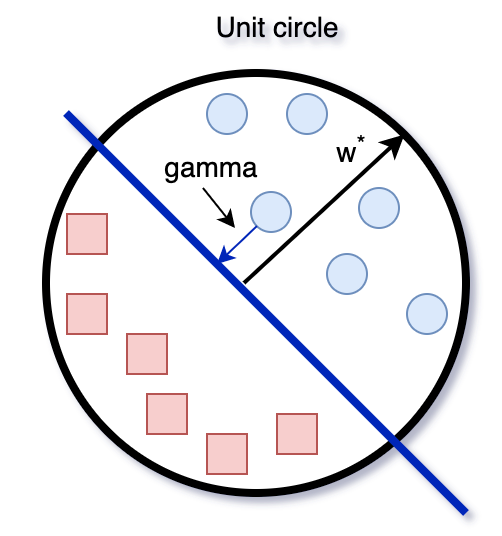
\includegraphics[width=0.3\textwidth]{Screen Shot 2022-06-02 at 16.20.41.png}
  %\caption{Illustration of a perceptron update}
  
\end{figure}
    
    
\end{frame}

\begin{frame}{Perceptron Convergence (cont.)}
    \underline{Theorem}: the Perceptron algorithm makes at most $\frac{1}{\gamma^2}$ updates.
    
    \underline{Proof}: Use two facts:
    $y(x^Tw) \leq 0$ $y(x^Tw^*) > 0$
    
    Consider the effect of an update ($w$ become $w+yx$) on two terms $w^Tw^*$ and $w^Tw$
    
    1. Consider the effect of an update on $w^Tw^*$
    $$(w+yx)^Tw^* = w^Tw^* + y(x^Tw^*) \geq w^Tw^* + \gamma$$
    The distance from the hyperplane defined by $w^∗$ to $x$ must be at least $\gamma$ (i.e. y(x^Tw^*) = |x^Tw^*| \geq \gamma)
    
    $\to$ $w^Tw^*$ \underline{grows by \textbf{at least} $\gamma$}
    
    2. Consider the effect of an update on $w^Tw$
    $$(w+yx)^T(w+yx) = w^Tw + 2y(w^Tx) + y^2(x^Tx) \leq w^Tw + 1$$
    The inequality follows from the fact that:
    \begin{itemize}
        \item $2y(w^Tx) < 0$ : $x$ was misclassified
        \item $0 \leq y^2(x^Tx) \leq 1$: $y^2$ = 1 and all $x^Tx \leq 1$ (because $||x|| \leq 1$) 
    \end{itemize}
    $\to$ $w^Tw$ \underline{grows by \textbf{at most} 1}
\end{frame}

\begin{frame}{Perceptron Convergence (cont.)}
    3. After $M$ updates:\\
    (1) $w^Tw^* \geq M\gamma$\\
    (2) $w^Tw \leq M$\\
    The proof:\\
    
    $M\gamma \leq w^Tw^*$ \quad \quad \quad \quad //by (1)\\[0.1cm]
    $ M\gamma \leq ||w||cos(\theta)$ \quad \quad //definition of inner-product\\[0.1cm]
    $ M\gamma \leq ||w||$ \quad \quad \quad \quad // $cos(\theta) \leq 1$\\[0.1cm]
    $M\gamma \leq \sqrt{w^Tw}$ \quad \quad \quad  // definition of $||w||$\\[0.1cm]
    $\quad \quad M\gamma \leq \sqrt{M}$\\[0.1cm]
    $\quad \quad M^2\gamma^2 \leq M$\\[0.1cm]
    $\quad \quad M \leq \frac{1}{\gamma^2}$
    
\end{frame}

\section{Support Vector Machine}
\begin{frame}{The Support Vector Machine (SVM)}
\begin{figure}[h!]
  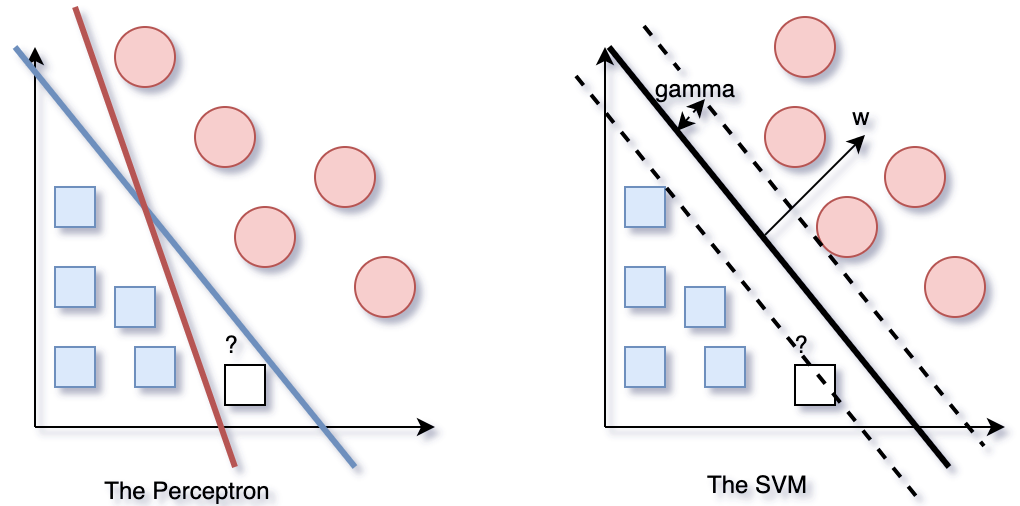
\includegraphics[width=0.5\textwidth]{Screen Shot 2022-06-02 at 18.02.31.png}
  %\caption{Illustration of a perceptron update}
\end{figure}
\underline{Question}: what is the best hyperplane?\\   
\underline{SVM}: the one that maximizes the distance to the closest data points from both classes.
    
\end{frame}

\begin{frame}{The SVM (cont.)}
\begin{minipage}{0.65\textwidth}
\textbf{Margin}: A hyperplane $H = \{x|w^Tx+b = 0\}$. Margin $\gamma$ defined as the distance from the hyperplane to the closest point across both classes. Let $d$ be the vector from $H$ to data point $x$ of minimum length. Let $x^p$ be the projection of $x$ onto $H$.
$\to x^p = x - d$\\
$d$ is parallel to $w$, so $d = \alpha w$, $x^p \in H$ which implies $w^Tx^p + b = 0$, therefore
$$w^Tx^p + b = w^T(x-d) + b = w^T(x-\alpha w) + b = 0$$
$\to \alpha = \frac{w^Tx+b}{w^Tw}$\\[0.1cm]
The length of d:\\
$$||d||_2 = \sqrt{d^Td} = \sqrt{\alpha^2w^Tw} = \frac{|w^Tx+b|}{\sqrt{w^Tw}} = \frac{|w^Tx+b|}{||w||_2}$$
$\gamma(w,b) = min_{x\in D}\frac{|w^Tx+b|}{||w||_2}$
\end{minipage}
\begin{minipage}{0.3\textwidth}

    \begin{figure}[h!]
  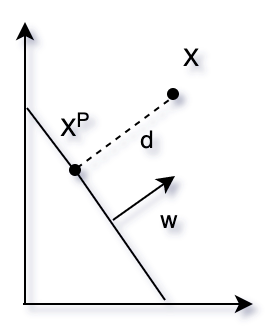
\includegraphics[width=0.7\textwidth]{Screen Shot 2022-06-02 at 21.33.43.png}
  %\caption{Linear classifier}
\end{figure}
\end{minipage}
    
\end{frame}

\begin{frame}{Max Margin Classifier}
Optimization problem:
\begin{itemize}
    \item $\textbf{max} \gamma(w,b)$ such that $\forall i: y_i(w^Tx_i + b) \geq 0$
    \item $\textbf{max}\frac{1}{||w||_2}\textbf{min}_{x_i\in D}|w^Tx_i + b|$
\end{itemize}
    
The hyperplane is scale invariant, we can fix the scale of $w$ and $b$ anyway we want.
$$min_{x\in D}|w^T+b| = 1$$
Objective:
$$\textbf{max}_{w,b}\frac{1}{||w||_2} = \textbf{min}_{w,b}||w||_2 = \textbf{min}_{w,b}w^Tw$$
s.t. $\forall i, y_i(w^Tx_i+b) \geq 0$ and $\textbf{min}|w^Tx_i + b| = 1$

$\to$ Quadratic optimization problem. The objective is quadratic and the constraints are all linear. 
\end{frame}


\section{Regression}

\begin{frame}{Linear Regression}
\begin{minipage}{0.55\textwidth}
\underline{Data assumption}: $y_i\in \textbf{R}$.\\
\underline{Model assumption}: $y_i = W^Tx_i$\\
\underline{Loss function}
$$l(W) = \frac{1}{n}\sum_{i=1}^{n}(W^Tx_i-y_i)^2$$
\begin{itemize}
    \item We estimate parameter $W^*$ to minimize a loss function $l(W)$: $w^* = argmin_w l(W)$
    \item This loss function known as the squared loss or Ordinary Least Squares (OLS).
    \item OLS can be optimized with gradient descent, Newton's method.
    \item Closed form: $\textbf{w}^* = (\textbf{XX}^T)^{-1}\textbf{X}\textbf{y}^T$ where $\textbf{X} = [\textbf{x}_1,...,\textbf{x}_n]$, $\textbf{y} = [\textbf{y}_1,...,\textbf{y}_n]$.
\end{itemize} 

\end{minipage}
\begin{minipage}{0.4\textwidth}

    \begin{figure}[h!]
  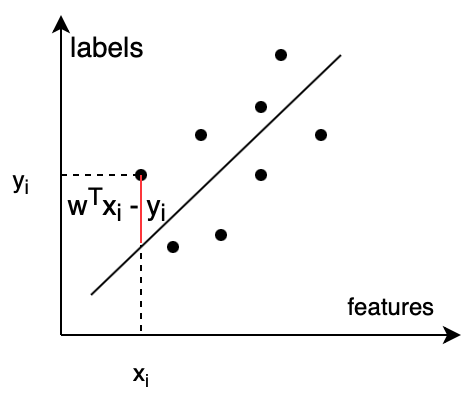
\includegraphics[width=0.7\textwidth]{Screen Shot 2022-05-21 at 17.19.06.png}
  \caption{Linear classifier}
\end{figure}
\end{minipage}
\end{frame}

\begin{frame}{Linear Regression (cont.)}
    Limitation of Linear Regression
    \begin{itemize}
        \item Sensitive to noise
        \item Cannot represent the complex models.
    \end{itemize}
    \begin{figure}[h!]
  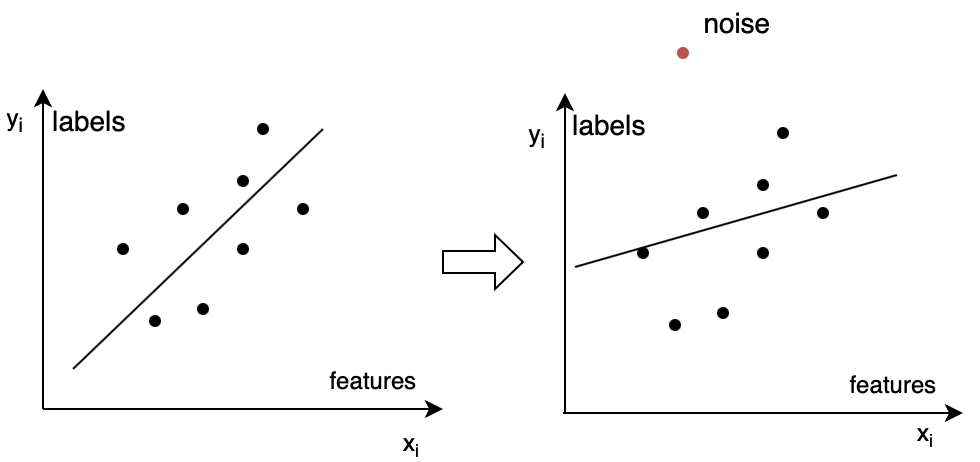
\includegraphics[width=0.7\textwidth]{Screen Shot 2022-05-21 at 18.04.04.png}
  %\caption{LR is sensitive to noise}
\end{figure}
\end{frame}

\iffalse
\section{Decision Trees}
\begin{frame}{Decision Trees}
    \begin{figure}[h!]
  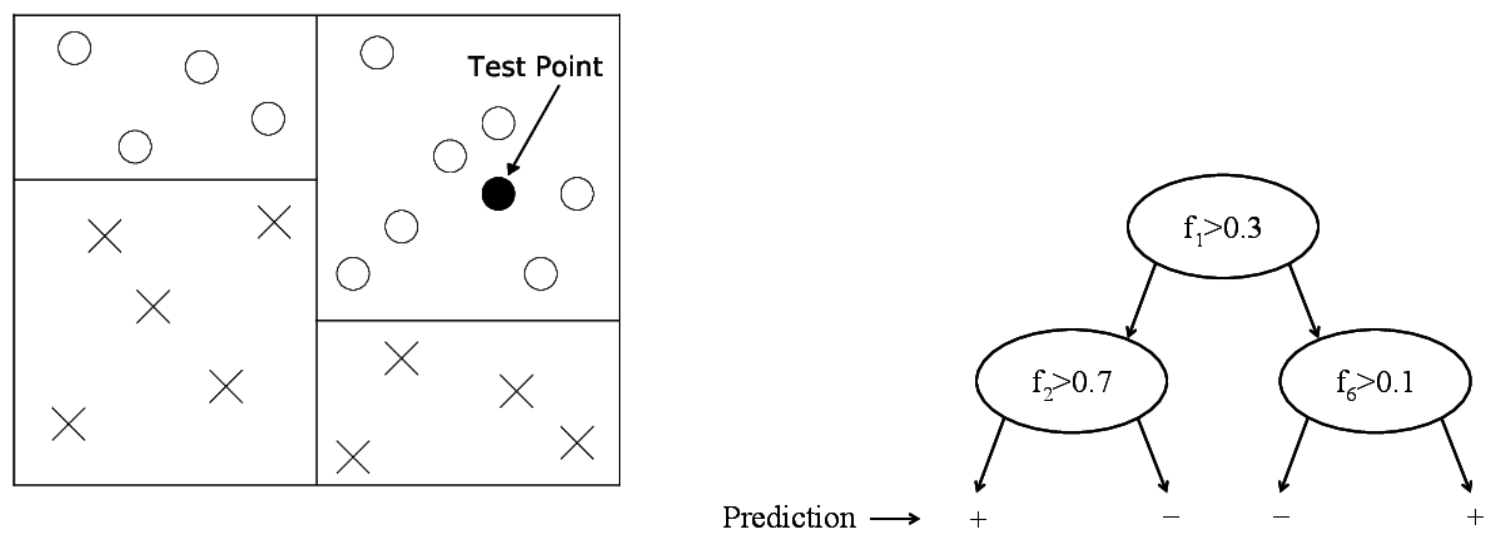
\includegraphics[width=0.7\textwidth]{Screen Shot 2022-06-24 at 22.57.21.png}
  \caption{Binary tree, only labels are stored}
\end{figure}
\underline{Goal}: Build a tree that is : \begin{itemize}
    \item Maximally compact
    \item Only has pure leaves
\end{itemize}
Is it always possible to find a tree? Yes, iff no two input vectors have identical features but differet labels\\
Minimize an \underline{Impurity function}: measures label purity amongst the children.

\end{frame}
\begin{frame}{Impurity Functions}
$S = \{(x_i, y_i)\}$, $y_i \in \{1, ..c\}$, c is the number of classes\\
Gini impurity\\
Let $S_k \subseteq S$ where $S_k = {x,y}\in S: y = k$ (inputs with label k), $S = S_1\cup S_2 \cup ... S_c$, \underline{define}:\\
$$p_k = \frac{|S_k|}{|S|}$$
Gini Coefficient of a leaf:
$$G(S) = \sum_{k=1}^{c} p_k(1-p_k)$$

 \begin{figure}[h!]
  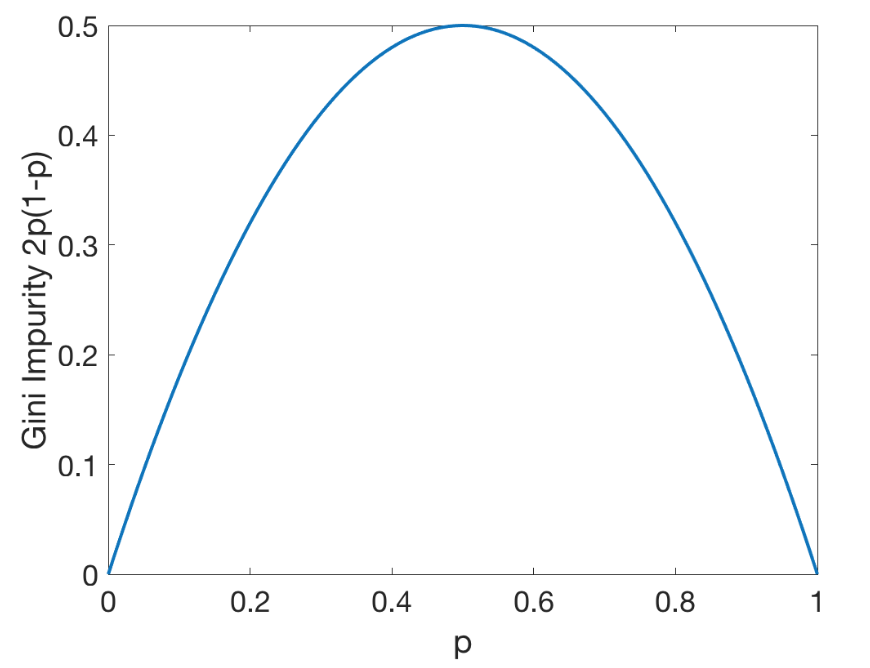
\includegraphics[width=0.3\textwidth]{Screen Shot 2022-06-24 at 23.14.55.png}
  \caption{p = 0.5}
\end{figure}
\end{frame}

\begin{frame}{Gini impurity of a tree}
$$G^T(S) = \frac{|S_L|}{|S|} G^T(S_L) + \frac{|S_R|}{S} G^T(S_R)$$
Where
\begin{itemize}
    \item $S = S_L \cup S_R$
    \item $S_L \cap S_R = \varnothing$ 
    \item $\frac{|S_L|}{|S|}$: fraction of inputs in left substree
    \item $\frac{|S_R|}{|S|}$: fraction of inputs in right substree
\end{itemize}
    
\end{frame}


\begin{frame}{Entropy}
    Let $p_1, ..., p_k$ be defined as before. We don't want $p_1 = p_2 =...= p_c = \frac{1}{c}$ (Uniform Distribution) $\to$ each leaf is equally likely $\to$ prediction is random guessing.\\
    Define the impurity as how close we are to uniform $\to$ use KL-divergence\\ Let $q_1, q_2, ..., q_c$ be the uniform distribution, i.e. $q_k = \frac{1}{c} \forall k$
    $$KL(p||q) = \sum_{c}^{k=1}p_k log\frac{p_k}{q_k} \geq 0$$
    $$ = \sum_{k}p_k log(p_k) - p_k log(q_k) = \sum_{k}p_k log(p_k) + p_k log(c)$$
    $$=\sum_{k}p_k log(p_k) + log(c) \sum_{k}p_k$$
    $$Max_{p}KL(p||q) = max_{p}\sum_{k}p_k log(p_k) = min_{p} - \sum_{k}p_k log(p_k)$$
    $$= min_{p}H(s) \leftarrow Entropy$$ 
    \underline{Entropy over tree}: $H(S) = p^LH(S^L) + p^RH(S^R)$, $p^L = \frac{|S^L|}{|S|}$ , $p^R = \frac{|S^R|}{|S|}$
\end{frame}

\begin{frame}{ID3}
    Base cases:\\
    ID3(S):\\
    If $\exists \hat{y}$ s.t. $\forall(x,y) \in S$, $y = \hat{y}$ return leaf with label $\hat{y}$\\
    If $\exists \hat{x}$ s.t. $\forall(x,y) \in S$, $x = \hat{x}$ return leaf with mode (y : (x,y) $\in$ S) or mean (regression)\\
    ID3 stop when:
    \begin{itemize}
        \item All the data points in a subset of have the same label.
        \item There are no more attributes could be used to split the subset. 
    \end{itemize}
    Try all features and all possible splits. Pick the split that minimizes impurity (e.g. s>t) where $f \leftarrow features$ and $t \leftarrow threshold$ \\
    \underline{Recursion}:\\
    Define: $S^L = \{S^L = \{(x,y)\ \in S: x_f \leq t\}\}$\\ \quad\quad Or:  
    $S^R = \{S^L = \{(x,y)\ \in S: x_f > t\}\}$
\end{frame}

\begin{frame}{Regression Trees}
    CART: Classification and Regression Trees\\
    \underline{Assumption}: labels are continuous: $y_i\ \in R$\\
   \underline{Impuriry: Squared Loss}\\
   Average squared difference from average label: $$L(S) = \frac{1}{|S|} \sum_{(x,y)\in S} (y-\hat{y}_S)^2$$ 
   $$\hat{y}_S = \frac{1}{|S|}\sum_{(x,y)\in S}y$$
   
\end{frame}

\section{Neual network}
\begin{frame}{Neural Network}
    It is also know as multi-layer perceptions and deep nets.\\
    
    \underline{Problem}: how can we make linear classifiers non-linear?\\
    \underline{Answer}: $w^T+b \to w^T \Phi(x)+b$\\
    Neural network learns $\Phi$:
    $\Phi(x)$ = \begin{bmatrix}
       h_1(x)           \\[0.3em]
       ... \\[0.3em]
       h_m(x)
     \end{bmatrix}
     Each $h(.)$ is a linear classifier. 
     \begin{figure}[h!]
  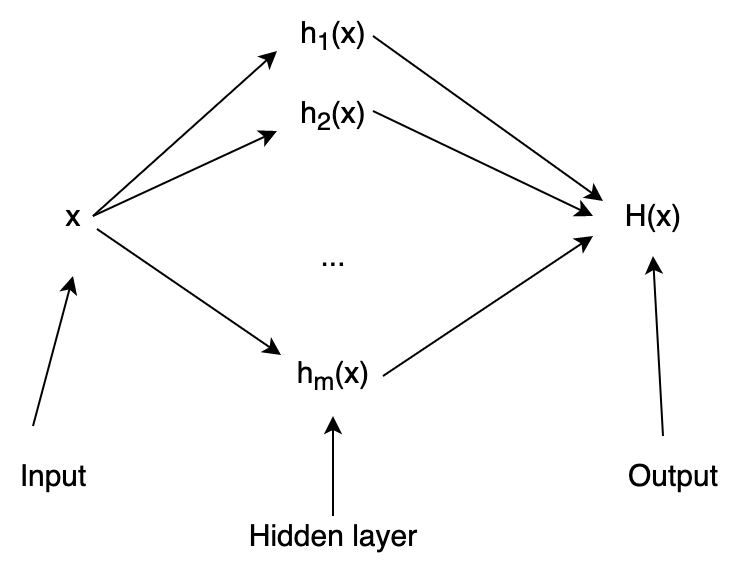
\includegraphics[width=0.3\textwidth]{Screen Shot 2022-06-25 at 11.41.37.png}

\end{figure}
\end{frame}

\begin{frame}{Neural Network}
    \begin{figure}[h!]
  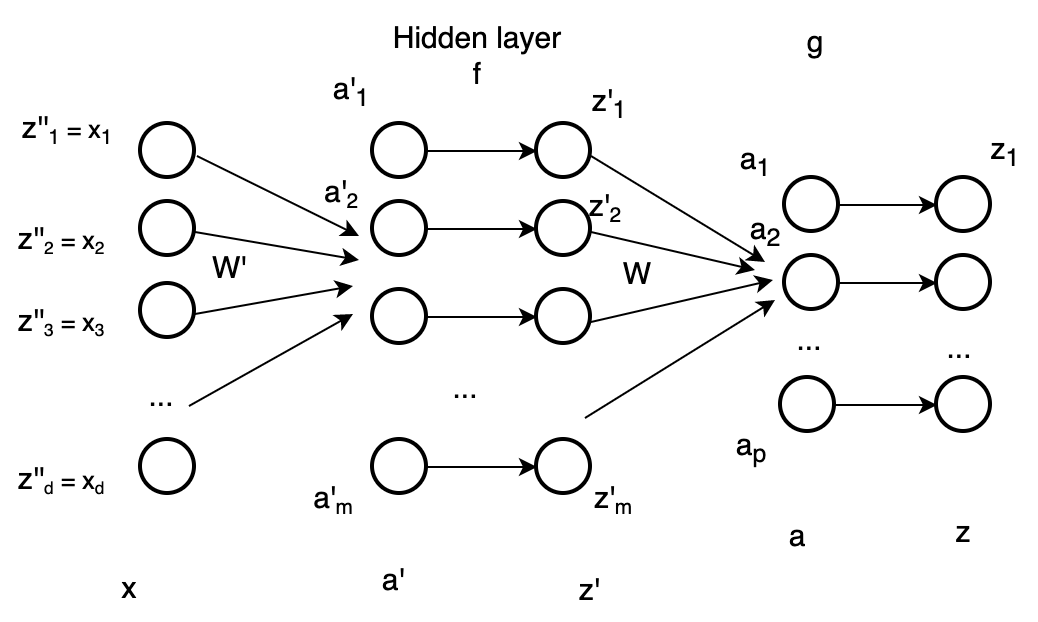
\includegraphics[width=0.4\textwidth]{Screen Shot 2022-06-25 at 12.01.05.png}
\end{figure}
$a'_j = \sum_{k} w'_{jk}+b'$\\
$a_j = \sum_{k} w_{jk}z'_j+b$\\
\end{frame}

\begin{frame}{Forward Propagation}
    Try to express $\Vec{z}$ in term of $w, w', b, b', f, y$ in matrix notation. We need to learn $w, w', b, b$.\\
    \underline{Back propagation}: Loss func for a single example:
    $$L(\Vec{x}, \Vec{y}) = \frac{1}{2}(H(\Vec{x} - \Vec{y}))^2$$
    where $H(\Vec{x}) = \Vec{z}$\\
    \underline{Observation}: chain rule\\[0.1cm]
    $\frac{\partial L}{\partial w_{ij}} = \frac{\partial L}{\partial \al}\frac{}{} = \frac{}{}$
\end{frame}


\section{Bagging}
\begin{frame}{Bagging}
    1. Sample $m$ data sets $D_1, ..., D_m$ from D with replacement\\
    2. For each $D_j$ train a classifier $h_j(.)$\\
    3. The final classifier is $h(x) = \frac{1}{m}\sum_{j=1}^{m}h_j(x)$.\\
In practice larger $m$ results in a better ensemble. Note that setting $m$ unnecessarily high will only slow down your classifier but will not increase the error of your classifier.
\end{frame}
\fi



\end{document}